\documentclass[tikz,border=2pt]{standalone}
\usepackage{amsmath,amssymb}
\usepackage{tikz}
\usetikzlibrary{arrows.meta}

\begin{document}
% The real number line: integers, fractions and irrationals such as sqrt 2, e and pi all have
% their place, and there are no gaps (completeness).
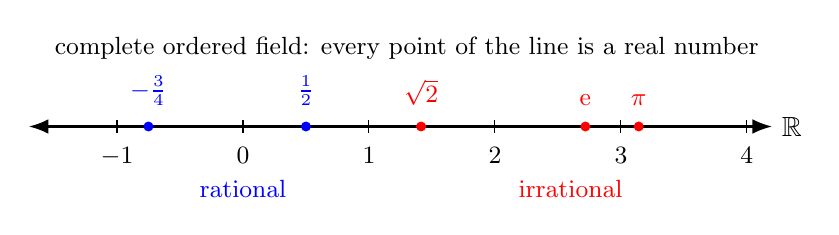
\begin{tikzpicture}[x=1.6cm]
	\draw[thick, {Latex[length=2.5mm]}-{Latex[length=2.5mm]}] (-1.7,0) -- (4.2,0);
	\node[right] at (4.2,0) {$\mathbb{R}$};
	\foreach \x in {-1,0,1,2,3,4} {\draw (\x,0.08) -- (\x,-0.08); \node[below=4pt, font=\small] at (\x,0) {$\x$};}
	\fill[blue] (0.5,0) circle (1.8pt); \node[blue, above=4pt, font=\small] at (0.5,0) {$\tfrac12$};
	\fill[blue] (-0.75,0) circle (1.8pt); \node[blue, above=4pt, font=\small] at (-0.75,0) {$-\tfrac34$};
	\fill[red] (1.414,0) circle (1.8pt); \node[red, above=4pt, font=\small] at (1.414,0) {$\sqrt2$};
	\fill[red] (2.718,0) circle (1.8pt); \node[red, above=4pt, font=\small] at (2.718,0) {$\mathrm{e}$};
	\fill[red] (3.1416,0) circle (1.8pt); \node[red, above=4pt, font=\small] at (3.1416,0) {$\pi$};
	\node[blue, below=16pt, font=\small] at (0,0) {rational};
	\node[red, below=16pt, font=\small] at (2.6,0) {irrational};
	\node[font=\small, above=18pt] at (1.3,0.1) {complete ordered field: every point of the line is a real number};
\end{tikzpicture}
\end{document}
